
\chapter{Thinking like an economist}

Every field of study has its own language and its own way of thinking.
The most important is to learn the economist's of thinking.


\section{The economist as scientist}

Economist try to address their subject with a scientist's objectivity:
\begin{itemize}
\item devise theories
\item collect data
\item analyze these data in an attempt to verify or refute their theories
\end{itemize}

\begin{tcolorbox}
  The essence of science is the scientific method -- the dispassinate development and testing of theories about how the world works.
\end{tcolorbox}

As Albert Einstein once put it, ``The whole of science is nothing more than the refinement of everyday thinking''.


\subsection{The scientific method: observation, theory, and more observation}



Although economists use theory and observation like other scientists, they do face an obstacle that makes their task especially challenging: Experiments are often difficult in economics.

\subsection{The role of assumptions}

Assumptions can make the world easier to understand.
The art in scientific thinking is deciding which assumptions to make.
Economists use different assumptions when studying the short-run and long-run efects of a change in the quantity of money.

\subsection{Economic models}

Economists use models that are most often composed of diagrams and equations to learn about the world.
Economic models omit many details to allow us to see what is truely important.
An economist's model does not include every feature of the economy.
All models are built with assumptions.
Economists assume away many of the details of the economy that are errelevant for studying the question at hand.
All models simplify reality in order to improve our understanding of it.

\subsection{The circular-flow diagram}

Circular-flow diagram: a visual model of the economy that shows how dollars flow through markets among households and firms.


\begin{figure}[!ht]
  \centering
  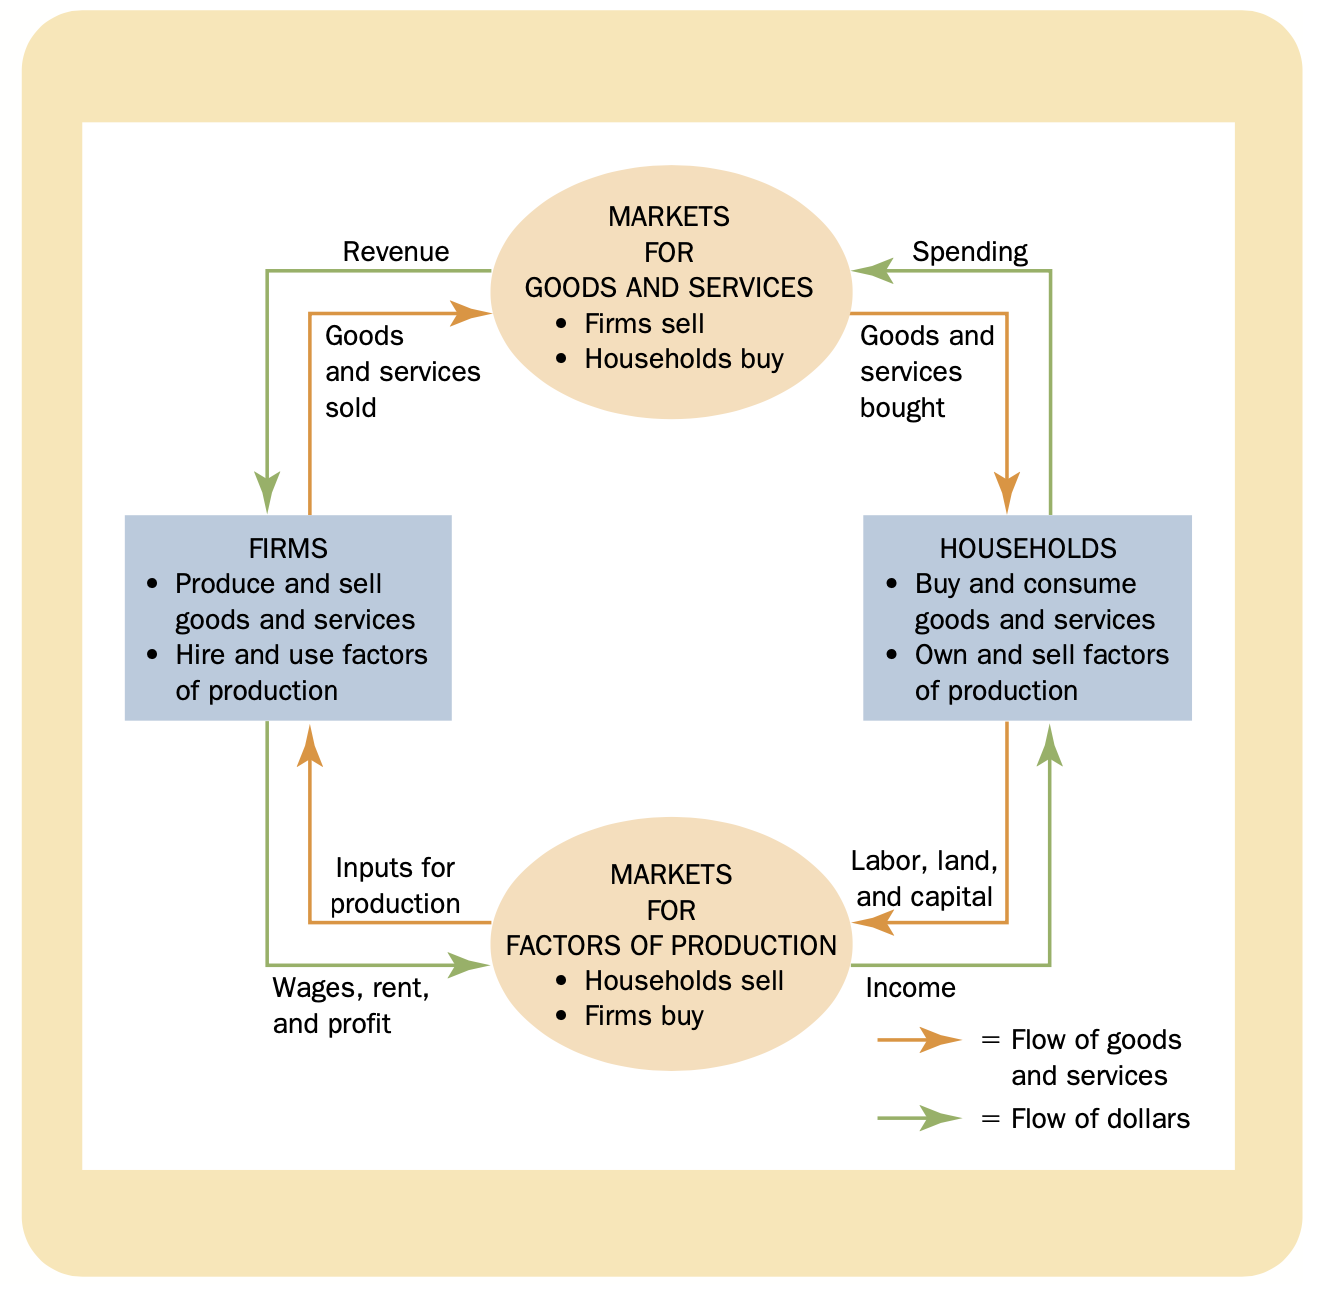
\includegraphics[width=\textwidth]{pics/circular-flow.png}
  \caption{The circular flow}
  \label{fig:circular-flow}
\end{figure}